\documentclass[11pt, a4paper]{article}

\usepackage[T1]{fontenc}
\usepackage[utf8]{inputenc}

\usepackage[english]{babel} %Hyphenation, titles, captions, tables in English (for more languages please refer to the babel manual)
\usepackage{csquotes} % Needed by babel
\usepackage{graphicx} %To include graphics
\usepackage{float} %Allows drawing of border around float - also used to define new float environments
\usepackage{endnotes} %Endnotes - footnotes that appear at the end.
\usepackage{pifont} %Font for picture symbols

\usepackage{booktabs}  %booktabs allows \toprule, \midrule, \bottomrule.
\usepackage{threeparttable} % threeparttable allows table notes, and adjusting the width of the caption to the width of the table


% With the next 3 parameters you can control the behaviour of latex how it handles floats and text. Normally it is not possible to fill a single page with only floats because LaTeX tries to achieve a certain text/float ratio per page. With these paremters this can be changed.

\renewcommand{\textfraction}{0.001} % having very little text on a page is OK
\renewcommand{\topfraction}{0.999}  % Having many floats in the upper half is OK
\renewcommand{\bottomfraction}{0.999} % Having many floats in the lower half is OK

% The omnipotent drawing package
\usepackage{tikz}

% Math packages
\usepackage{amsmath} 
\usepackage{amsfonts}
\usepackage{amssymb}

% Change page dimensions/borders
\usepackage[top=2.5cm, left=2cm, right=2.5cm, bottom=2cm]{geometry}
\usepackage{a4}

% Index directory
\usepackage{makeidx}
\makeindex

% Bibliography packages
\usepackage[style=authoryear, backend=biber, maxnames=5]{biblatex}
\addbibresource{bibliography.bib}



\pagestyle{headings} %standard headings. other options: plain, empty


% Custom command
\newcommand{\ltx}{\LaTeX}

%\linespread{1.2}\selectfont % Global Zeilenabstände ändern

\setlength{\belowcaptionskip}{2ex}
\setlength{\abovecaptionskip}{1ex}

% Redefinition of margin parameters
% More information: http://tex.stackexchange.com/questions/48571/redefine-marginpar-with-renewcommand
\let\oldmarginpar\marginpar
\renewcommand{\marginpar}[1]{\oldmarginpar{\textit{#1}}}




% Title page
\title{\ltx{} made easy}
\author{John Doe\\ University Here\thanks{john.doe@uni-here.edu} \and Michael Smith\\University there\thanks{michael.smith@uni-there.edu}}

% Should be loaded last to avoid overwriting of package settings
\usepackage{hyperref} %Creates clickable references in the document - ideally loaded last in the document preambel

%%%%%%%% BEGIN OF DOCUMENT %%%%%%%%
\begin{document}

\maketitle
\tableofcontents
\newpage

\section{Easier than its reputation}

For a ``simple'' \ltx-document only a handful of commands are needed. You do not even have to care aboutr formatting but can instead completely focus on the text.

Apart from a few special characters, the majority of the text can be typed as you usually do.

\section{Simple text formatting}

A new paragraph can be produced if you insert at least one empty line. It does not matter whether it is one or many empty lines it all ends up creating just a simple new paragraph. So unlike in Word you can not format your documents with many new lines. Same applies to spaces: one or many spaces always only insert a simple space.

\subsection{Hyphenation and dashes}

You do not have to care about hyphenation. \ltx\ will take care of this. However if there is a word that you want to have hyphenated differently, there are options to achieve this.

There are different types of dashes. The normal dash (-) -- used to connect words -- and the double dash: -- which is just 2 consecutive dashes or the long version of this (---) (3 consecutive dashes).


\subsection{Quotations}
Quotation marks\index{Quotations} are set with \`{}\`{} \verb+''+ (`` ''). For German quotes use "\`{} "\verb+'+ ("` "') or for French \verb+"< ">+ ("< ">).

\begingroup
\setlength{\parindent}{0pt}
\setlength{\parskip}{1.5ex plus 0.5ex minus 0.2ex}
\section{Text formatting\label{sec:eftf}}

\subsection{Characters}

\subsubsection{Special characters}
If you want to use non ASCII characters (like é or ł ą ę) it is recommended to use UTF8 encoded input and a font that also supports these characters (most fonts support characters used in French, Polish, Italian and others). This is also why the document loads \texttt{fontenc} and \texttt{inputenc} with the option \texttt{T1} and \texttt{utf8} respectively.

\subsection{Paragraphs}
This text contains both paragraphs and simple new lines. For section \ref{sec:eftf} (starting on page \pageref{sec:eftf}) it has been set that for the first line of every paragraph there is no indentation.

\begingroup
\raggedright % Left justified
The spacing between paragraphs should be 1.5\,ex, can be extended at most by 0.5\,ex and reduced by at most 0.2\,ex. This paragraph and the next should be left justified. 

\vspace{1cm}
\subsection{Misc.} 
An \fbox{additional} $1$\,cm has been inserted before this paragraph.
\endgroup
\endgroup

\section{Visual formatting}
Most of the formatting done in section~\ref{sec:eftf} \nameref{sec:eftf} are of visual nature i.e. the commands describe how the text should look like. For all practical purposes you ideally should not use these kinds of commands (of course there are justified exceptions). It is better to use logical formatting which describes the significance a part of the text has with respect to the document structure or its content.

\section{Fonts in \ltx}

The font style in \ltx{} is defined by 3 features:

\begin{enumerate}
\item Font family
\begin{itemize}
\item Fonts with serifs (roman): proportional fonts with small helper lines attached to each letter.
\item \textsf{Sans serif fonts: proportional fonts without helper lines}.
\item \texttt{Typewriter fonts: mono spaced font}.
\end{itemize}
\item Font weight:
\begin{itemize}
\item normal weight
\item \textbf{bold weight\index{fett|textbf}}
\end{itemize}
\item Form of the font:
\begin{itemize}
\item Upright fonts
\item \textsl{Slanted fonts}
\item \textit{Italic fonts}
\item \textsc{Small caps}
\end{itemize}
\end{enumerate}

Even though there are many options to manipulate font face, weight and style there is one rule you should always remember:
\begin{quote}
Typography is a trade that has to be learned. Someone not trained in this often makes disastrous mistakes. Many people mistakenly believe that the design of a text is mostly aesthetics and a ``nice look'' is the ultimate goal -- which is a mistake. A text is to be read and not to be wondered at in a museum. Readability and intelligibility are much more important than the ``nice looks''.
\end{quote}

\noindent Here a few pointers that you should consider when you write your text:
\begin{itemize}
\item[\ding{43}] Extensive texts should be set with a serif font.
\item[\ding{43}] Highlighting in a text can be done with \textsl{slanted} or \textit{italic} form. Italic fonts highlight better than slanted. Really important parts can be highlighted with \textbf{bold} faced text.
\item[\ding{43}]  \textsf{Text sans serif are suitable for headers and titles}
\item[\ding{43}] Less is more: Do not try to over design your text. Leave most work to \ltx.
\end{itemize}


\begin{table}[t]
\caption{Example table  \label{tab:Schriftgroessen}}
\centering
\begin{tabular}{lccc}
\toprule
\textbf{\ltx-Command} & \multicolumn{3}{c}{\textbf{Base size}}\\
\cline{2-4} & \textbf{10\,pt} & \textbf{11\,pt} & \textbf{12\,pt}\\
\midrule
\midrule
\verb+\tiny+			& 5\,pt & 6\,pt 	& 6\,pt\\
\verb+\scriptsize+		& 7\,pt & 8\,pt		& 8\,pt\\
\verb+\footnotesize+	& 8\,pt & 9\,pt		& 10\,pt\\
\verb+\small+			& 9\,pt & 10\,pt	& 11\,pt\\
\midrule
\midrule
\verb+\normalsize+		& 10\,pt	& 11\,pt	& 12\,pt\\
\midrule
\midrule
\verb+\large+			& 12\,pt	& 12\,pt	& 14\,pt\\
\verb+\Large+			& 14\,pt	& 14\,pt	& 17\,pt\\
\verb+\LARGE+			& 17\,pt	& 17\,pt	& 20\,pt\\
\verb+\huge+			& 20\,pt	& 20\,pt	& 25\,pt\\
\verb+\Huge+			& 25\,pt	& 25\,pt	& 25\,pt\\
\bottomrule
\end{tabular}
\end{table}%

\section{Table example}
Table \ref{tab:Schriftgroessen} shows the font size for the \ltx font size commands with respect to their base font size.

The smallest font size is 5~pt the largest 25~pt.

\section{Images in \ltx}
\ltx{} allows the creation of graphics directly with \ltx commands as embedding external image files. Both option will be shown in the following examples.

\subsection{Line figures with \ltx commands}

\ltx{} allows the creation of plots directly via \ltx-commands. One example can be seen in fig.~\ref{fig:tikz}. Tikz is an additional package like many which has to be loaded in the
preamble. With Tikz one has endless possibilities, all you need is an idea how to put it to paper. For more information please read \textit{A very minimal introduction to Tikz} (\url{http://cremeronline.com/LaTeX/minimaltikz.pdf}).
%
\begin{figure}[t]
\centering
\begin{tikzpicture}[scale=0.6]
% Create coordinate system
\draw [->] (-5,0) -- (5,0);
\draw [->] (0,-5) -- (0,5);

% Label axis
\node [below] at (5,0) {$x$};
\node [left] at (0,5) {$y$};

% Repeat vertical line in the 1. quadrant
\foreach \x in {0.25, 0.5, 0.75,...,3} {
\draw (\x, 0) -- (\x, 3);
}

% The rectangle: cycle connects the last point with the first.
\draw (-3,-3) -- (-3,3) -- (3,3) -- (3,-3) -- cycle;

% Diagonal line
\draw (-4,-4) -- (4,4);

% Separation of the coordinate axis
\foreach \t in {-4,-3,...,4}{
\draw (\t, -0.2) -- (\t, 0.2);
\draw (-0.2,\t) -- (0.2,\t);
}
\end{tikzpicture}
\caption{A Tikz figure\label{fig:tikz}}
\end{figure}


\subsection{Some history -- embedding of pictures}
In the beginning there was a book project. IT professor Donald Knuth typeset the first volume of his book ``The Art of Computer Programming'' 1969 with \textit{Monotype} a technology from the 19\(^{\text{th}}\) century. In 1976 when the second volume was about to be published, most of the monotype technology has been replaced by photographic typesetting. When Knuth received the pages to proofread he thought them to be awful and thus he began in 1977 to write his own typesetting system -- \TeX was born.

\begin{figure}[htb]
\centering
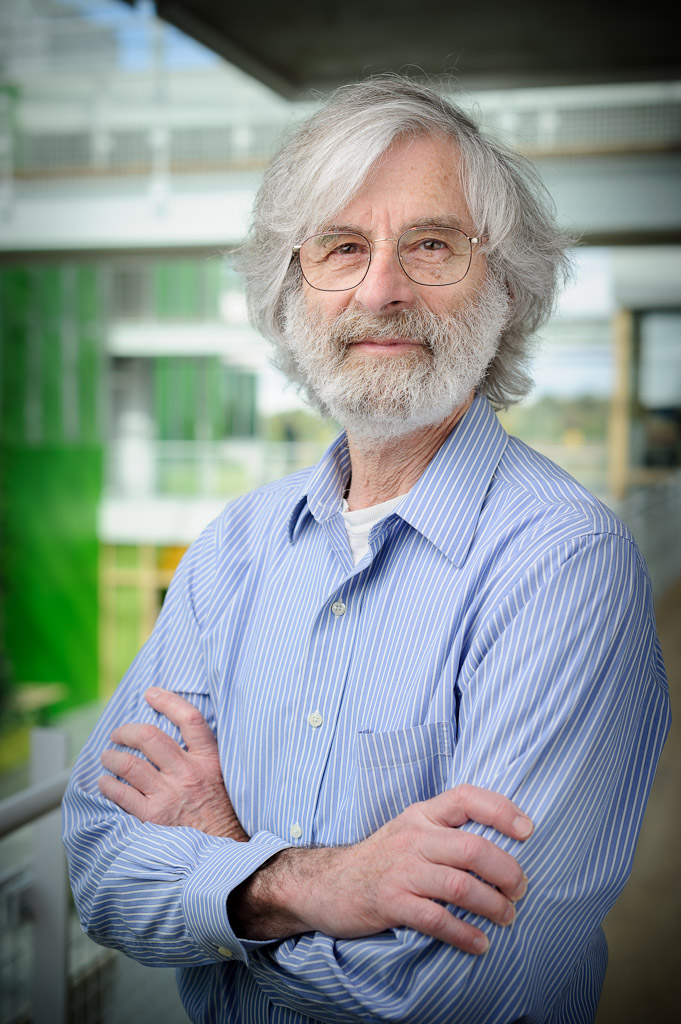
\includegraphics[width=0.3\textwidth]{Leslie_Lamportd}
\caption{Leslie Lamport\label{fig:LL}}
\end{figure}

\TeX{} offers many option for text formatting but it is difficult and cumbersome to use. Leslie Lamport, an American computer scientist believed that an author should focus on content and not formatting. In 1984 he began writing a macro package for \TeX{} which takes responsibility for many formatting decisions and many other simplifications -- \ltx.

\section{Basics of math typesetting}

Scientific papers with a lot of formulas set a high requirement to the typesetting system because mathematical expressions and formulas should be treated differently that running text. One emphasis of the development of \TeX{} and \ltx{} was on a high-quality for the mathematical typesetting to be in accordance with the conventions.

\begingroup
\floatstyle{boxed}
\restylefloat{figure}
\begin{figure}[p!] %p erzielt, dass die figure auf einer Seite speziell für floats platziert wird
Given the family of functions
\begin{displaymath}
f_a(x) = \frac{x+a}{x^2}~\mbox{mit } a \in \mathbb{R}
\end{displaymath}
\begin{enumerate}
\item Investigate the family of functions \( f_a\) for it's maximum domain \(\mathbb{D}\). Determine the asymptotes for the graphs as the behavious of the graphs at the border of the domain.
\item Proof that for two different graphs of the family there is no intersection but they approach each other arbitrary close at \(x\to\infty\).
\item Draw the graph \(G_{f_1}\) in the range \(I = \left[-4;4\right]\) in a suitable coordinate system.
\item Show that
\begin{displaymath}
F(x) = x +(x+1)\cdot\ln(x+1) - 2x\cdot\mbox{ln}(x)
\end{displaymath}
is a primitive of \(\displaystyle g(x) = \ln\left(\frac{x+1}{x^2}\right)\) is.
\end{enumerate}
\caption{A simple maths sheet}
\label{fig:formeln}
\end{figure}
\endgroup

Part of the mathematical typesetting are:
\begin{itemize}
\item Numbers, variables and operators
\item Mathematical symbols
\item Name of functions
\item Greek letters
\item Indices and exponents
\item Complete mathematical formulas
\item various special characters.
\end{itemize}

Numbers and operators are set in an upright style, variables mostly italic without kerning.

A very important package for typesetting formulas is developed by the American Mathematical Society (\AmS) called \textit{amsmath} which in addition to operators and symbols also offers additional structuring elements and design possibilities. It is a good idea to load this package in any preamble (\verb+\usepackage{amsmath}+).

Fig.~\ref{fig:formeln} shows a selection of formulas. Also it shows that a figure environment is not necessarily only for figures.

\clearpage %beginnt eine neue Seite und platziert alle noch nicht gesetzten Floats

\section{Footnotes and margin notes}

Following a quote from a textbook, suitably annotated with footnotes\marginpar{Footnotes}

\begin{quote}
Longer, additional explanations are often not placed within the running text since context can get lost quickly. Rather we set a marking -- often a raised number\footnote{often in increasing order} -- which refer to the explanation\footnote{be aware that too many footnotes can disturb the reading rhythm as well. Always consider if you really need this annotation and if you cannot keep it in the running text.}. In the footer this number will be repeated and the corresponding text will be typeset in a smaller font size\footnote{font size \texttt{footnotesize}}. For a clear separation between running text and footnotes a small horizontal line will be place between the two\footnote{some publications have a line across the whole page even.}.

It is quite simple to place footnotes in the running text. The numbering is handled automatically by \ltx{}. If you add more footnotes or delete some later the numbering will automatically be updated\footnote{Furthermore, \ltx{} also manages the page on which the footnote will appear which should always appear on the same page as the raised number. \ltx{} succeeds at this most of the time (except under some tricky circumstances) whereas Microsoft Word fails here above average.}. The numbering will be reset after every chapter (this concerns the document classes \textit{report} and \textit{book}). 

\end{quote}

Another way to handle additional explanations are \textit{endnotes}\marginpar{endnotes}. Compared to footnotes endnotes can be gathered and placed at the end of a chapter or even at the end of a document. Especially with longer annotations or many small annotations per page it can be sensible to use endnotes instead of footnotes. In order to being able to use endnotes a package is needed: \texttt{endnotes}.

Marginalia\marginpar{Marginalia} are also annotations in a sense. However these are of the shorter kind, small indicators to hint at something within the running text.

\section{Bibliography with Bib\LaTeX}

To create a bibliography with Bib\ltx{} a separate database file is recommend in which all the sources are listed with the respective data (author, year, publisher, etc.). 

You will create your references in a .bib file (essentially a text file) with a 3rd party program. There are many different programs that can help with creating these references, for this course we will use \textit{Jabref} a program based on Java so it is running on any operating system.

Once you have your database file, Bib\ltx{} will perform following tasks for you:
\begin{itemize}
\item Creating a list of all the cited sources in the document
\item Support of adding additional non-cited sources
\item Applying a bibliography style (can be custom made but this is not trivial and goes beyond the scope of this course)
\item Sorting the references according to style
\item Syntax check of the bibliography file
\item Checking the uniqueness of the keys
\end{itemize}


\section{Indices}
Leslie Lamport, author of \ltx{}, on indices:
\begin{quote}
A list of indices should make the finding of information in the document as easy as possible for the reader. Many authors are indexing the same words on every page where this word appears. A better approach would be to set the indices according to ideas, facts and concepts.

For the creation of an index you should decide which concepts you want to list. Then you should decide for which key words a reader is most likely to search for, to find this concept. 

You might be tempted to create the indices during the writing of your text. Try to resist this urge -- it is better to do this once the text and all the appearing concepts are finished and you have a clear idea how you want to index these concepts.
\end{quote}


\begin{table}[h!]
\centering
\caption{Overview of indexing commands\label{tab:Indexbefehle}}
\begin{tabular}{lll}
\toprule
Example &	Index Entry	 & Comment\\
\midrule
\verb+\index{hello}+ &	hello, 1	& Plain entry \\
\verb+\index{hello!Peter}+	&  Peter, 3	 &Subentry under 'hello'\\
\verb+\index{Sam@\textsl{Sam}}+&	\textsl{Sam}, 2	&Formatted entry\\
\verb+\index{Lin@\textbf{Lin}}	+&	\textbf{Lin}, 7	&Same as above\\
\verb+\index{Jenny|textbf}+&	Jenny, \textbf{3}	&Formatted page number\\
\verb+\index{Joe|textit}+&	Joe, \textit{5}	&Same as above\\
\verb+\index{ecole@\'ecole}+&	école, 4&	Handling of accents\\
\verb+\index{Peter|see{hello}}+&	Peter, \textit{see} hello	&Cross-references\\
\verb+\index{Jen|seealso{Jenny}}+ &	Jen, \textit{see also} Jenny	&Same as above\\
\bottomrule

\end{tabular}

\end{table}%

\newpage

\printbibliography
\printindex
\end{document}
